\documentclass[runningheads,a4paper]{llncs}

%
\usepackage{amssymb}
\usepackage{amsmath}
\usepackage{url}
\usepackage{graphicx}
\usepackage{multirow}
\usepackage{wrapfig}
%
\newcommand{\argmin}[1]{\underset{#1}{\operatorname{arg}\operatorname{min}}\;}
\setlength{\belowcaptionskip}{-15pt}
\setlength{\abovecaptionskip}{-2pt}
%
\mathchardef\mhyphen="2D
\raggedbottom 
%
% Allow easy processing of labeled images in figures
\newcounter{lfigcounter}
\newenvironment{IonTab}{\begin{table}[htb]}{\end{table}}
\newenvironment{IonFig}{\setcounter{lfigcounter}{1}\begin{figure}} {\end{figure}}
\newenvironment{IonFigH}{\setcounter{lfigcounter}{1}\begin{figure}[h]}{\end{figure}}
\newenvironment{IonFigT}{\setcounter{lfigcounter}{1}\begin{figure}[!t]}{\end{figure}}
\newenvironment{IonFigB}{\setcounter{lfigcounter}{1}\begin{figure}[b]}{\end{figure}}
\def\ionbox#1{\makebox[#1]{(\alph{lfigcounter})}\stepcounter{lfigcounter}}
%
\begin{document}

\mainmatter  % start of an individual contribution

% first the title is needed
\title{An Image-based method for phase estimation, gating and temporal super-resolution of \\cardiac ultrasound}

% a short form should be given in case it is too long for the running head
\titlerunning{An Image-based Phase Estimation Method for Cardiac Ultrasound}

% the name(s) of the author(s) follow(s) next
%
% NB: Chinese authors should write their first names(s) in front of
% their surnames. This ensures that the names appear correctly in
% the running heads and the author index.
%

% anonymous stuff
\author{*}
\authorrunning{*}   
\tocauthor{*}
\institute{*}

\maketitle

\begin{abstract}
Ultrasound is emerging as an increasingly effective tool for rapid non-invasive assessment of cardiac structure and function. Knowledge of the phase or location of each video frame within the cardiac and/or respiratory cycles is essential in many applications. In this paper, we present a novel method for estimation of instantaneous cardiac and respiratory phases directly from cardiac ultrasound videos. The method transforms the complex high-dimensional image sequence into a univariate time series with the same periodicity characteristics, decouples the periodic sources of beating heart and respiratory motion using a trend extraction technique, and estimates the cardiac and respiratory phases using the Hilbert transform. We also present a robust non-parametric regression technique for gating out respiratory frames and a novel kernel regression model that reconstructs images at any cardiac phase and facilitates temporal super-resolution. We validate our methods using cardiac ultrasound or echocardiography videos and ECG recordings of 6 mice.
%\keywords{Cardiac, Ultrasound, Echocardiography, Phase estimation, Gating, Temporal Super-resolution}
\vspace{-0.5cm}
\end{abstract}
%
\section{Introduction}
\label{sec:intro}
%
Cardiovascular disease is the leading cause of death worldwide and ultrasound is emerging as an increasingly effective tool for rapid non-invasive assessment of cardiac structure and function. Cardiac ultrasound videos consist of two kinds of periodic motion, one corresponding to beating heart motion and the other corresponding to respiratory motion. Knowledge of the phase or location of each video frame within the cardiac and/or respiratory cycles is essential in a variety of applications such as gating\cite{VonBirgelen1997}, quiescence detection\cite{Wick2013}, 3D reconstruction\cite{Wachinger2012}, and temporal super-resolution\cite{Cherin2006}. Typically, the position within cardiac cycle is tracked through ECG data and position within respiratory cycle is tracked by motion of markers placed on the subject's body\cite{Khamene2004}. 

	In this paper, we present a novel method that estimates the instantaneous cardiac and respiratory phases directly from the cardiac ultrasound video. We also present a robust non-parametric regression technique for gating out respiratory frames and a novel kernel regression to reconstruct images at any cardiac phase to facilitate temporal super-resolution. Previous work on the estimation of cardiac and/or respiratory phases directly from ultrasound videos is very limited. In~\cite{Karadayi2006}, the authors compute a signal measuring the x- or y-coordinate of the center of mass of each frame, use bandpass filtering to remove components outside typical cardiac frequency range, find the dominant frequency and apply matched sine/cosine filters to estimate the instantaneous phase. In~\cite{Sundar2009}, the authors compute a signal measuring phase correlation between consecutive frames, use a bandpass filter centered at 1Hz to recover the cardiac signal, and use a low pass filter to recover the respiratory signal.
%
\vspace{-0.5cm}
\section{Method}
\label{sec:method}
%
In this section, we present the theory underlying the proposed methods. Specifically, we begin by describing our method for the estimation of instantaneous cardiac and respiratory phases in Section \ref{sec:method:phase_estimation}. We then present a robust method that uses these phase estimates to gate out video frames with significant respiratory motion in Section \ref{sec:method:gating}. Finally, in Section \ref{sec:method:super_resolution}, we present a kernel regression model for reconstructing images at any cardiac phase and facilitate temporal super-resolution.
%
%
\begin{IonFigT}
\centering
%
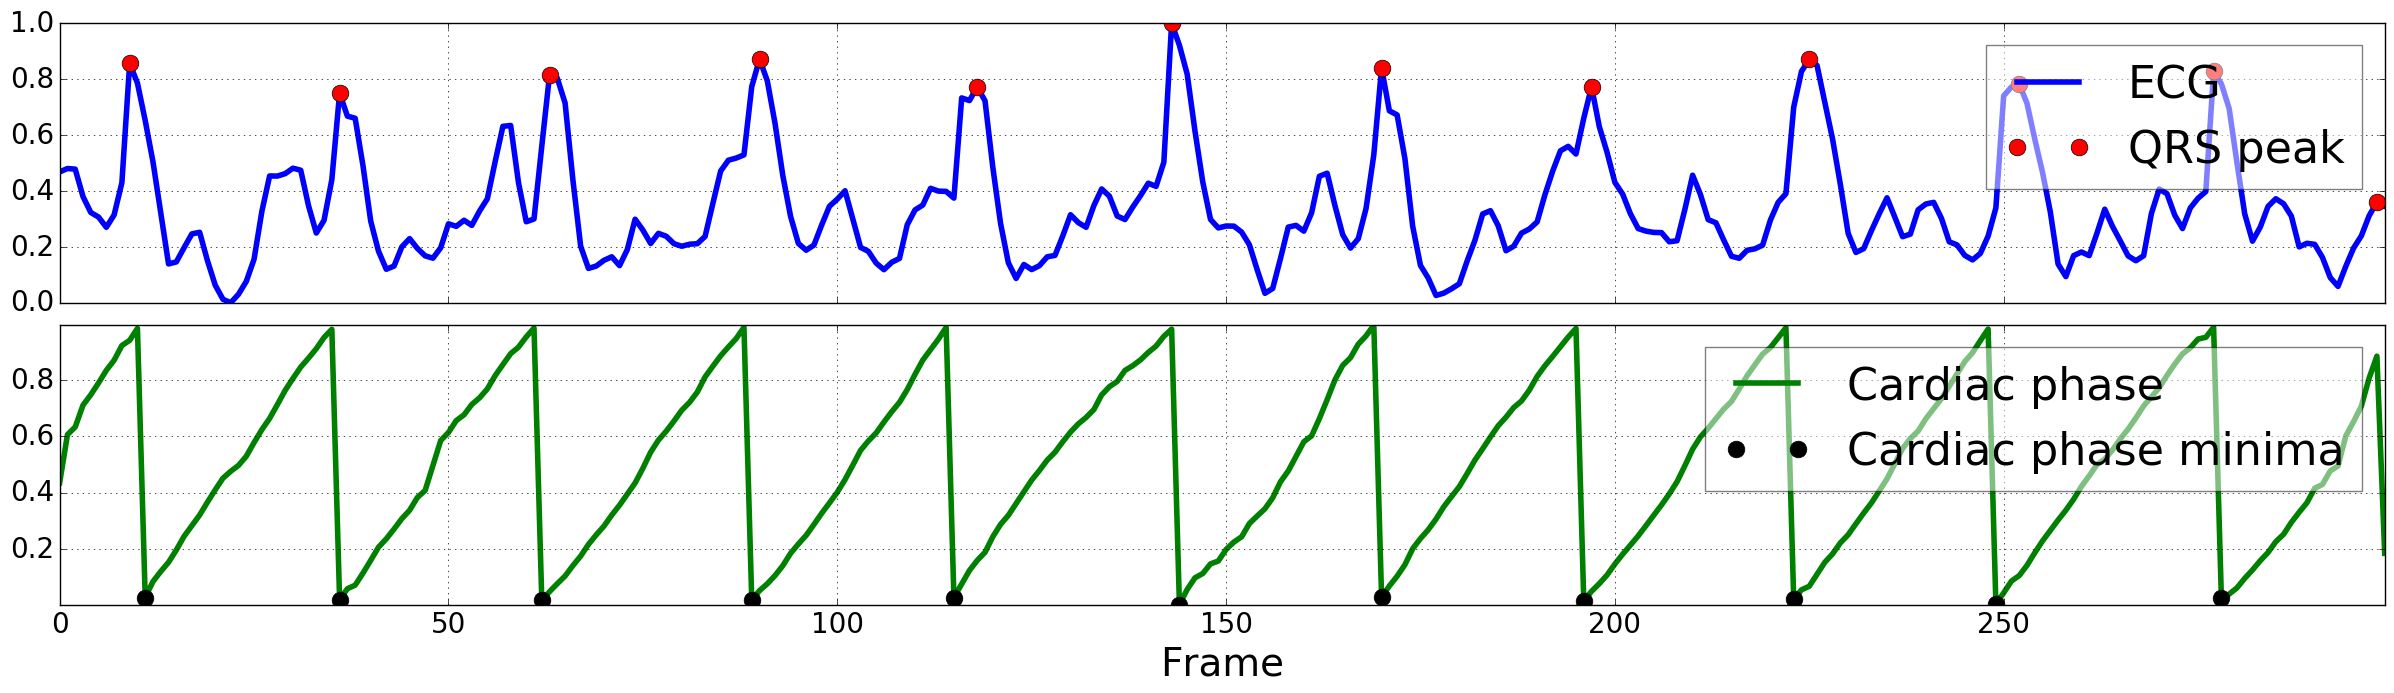
\includegraphics[width=4.5in]{figures/decoded/2015-07-27-10-36-06_2015-07-15-16-56-16_1.raw.bmode/ecg_instaphase_overlay.png}\\
\ionbox{4.5in}\\
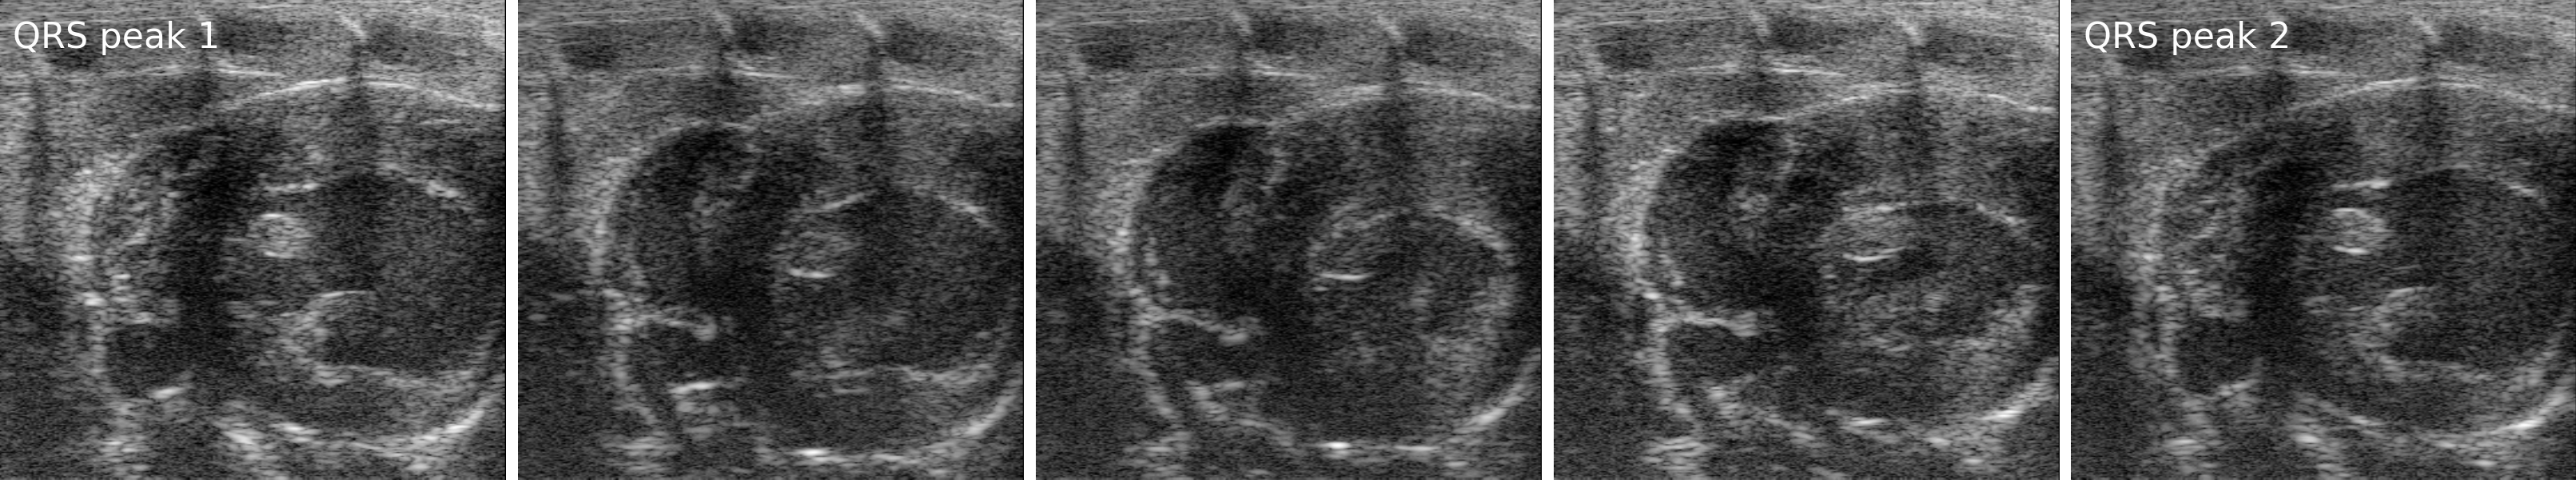
\includegraphics[width=4.5in]{figures/decoded/2015-07-27-10-36-06_2015-07-15-16-56-16_1.raw.bmode/qrs_peak_to_peak.png}\\
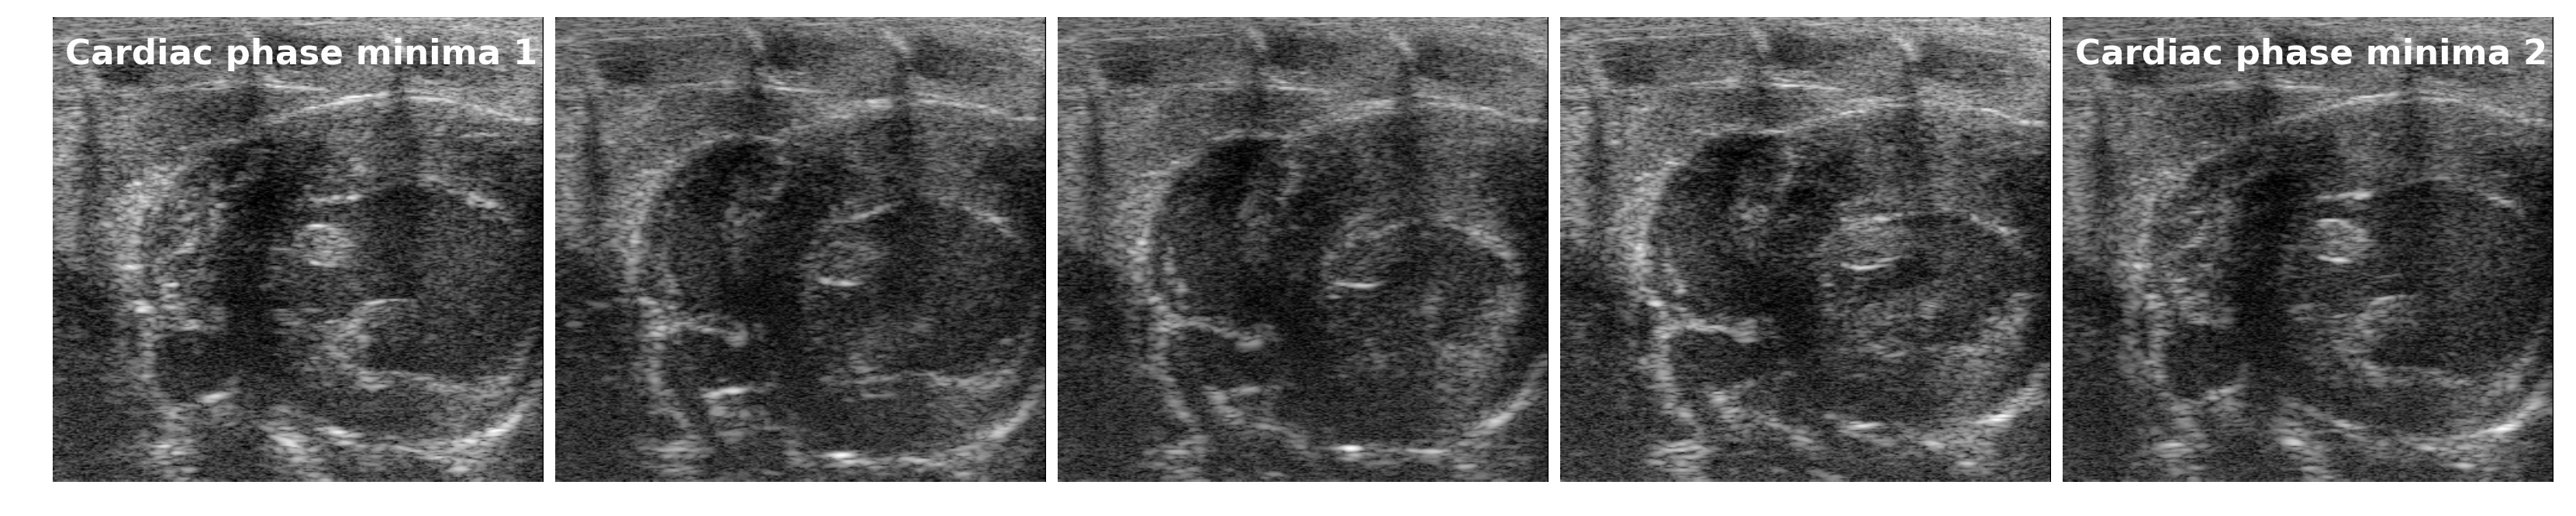
\includegraphics[width=4.5in]{figures/decoded/2015-07-27-10-36-06_2015-07-15-16-56-16_1.raw.bmode/instaphase_valley_to_valley.png}
\ionbox{4.5in}\\
%
\caption{Illustration of correspondence between ECG and the instantaneous cardiac phase estimated using our method: (a) ECG signal (blue) and the cardiac phase estimated using our method overlaid with peaks of the QRS complex (red circle) and the corresponding cardiac phase minima (black circle), (b) Five video frames evenly spaced in time between the first and second QRS peaks of the ECG signal (top-row) and the corresponding cardiac phase minima (bottom-row) constituting one cardiac cycle.}
\label{fig:instaphase_vs_ecg}
\end{IonFigT}
\vspace{-0.5cm}
\subsection{Estimation of instantaneous cardiac and respiratory phases}
\label{sec:method:phase_estimation}
%
\begin{IonFigT}
\centering
%
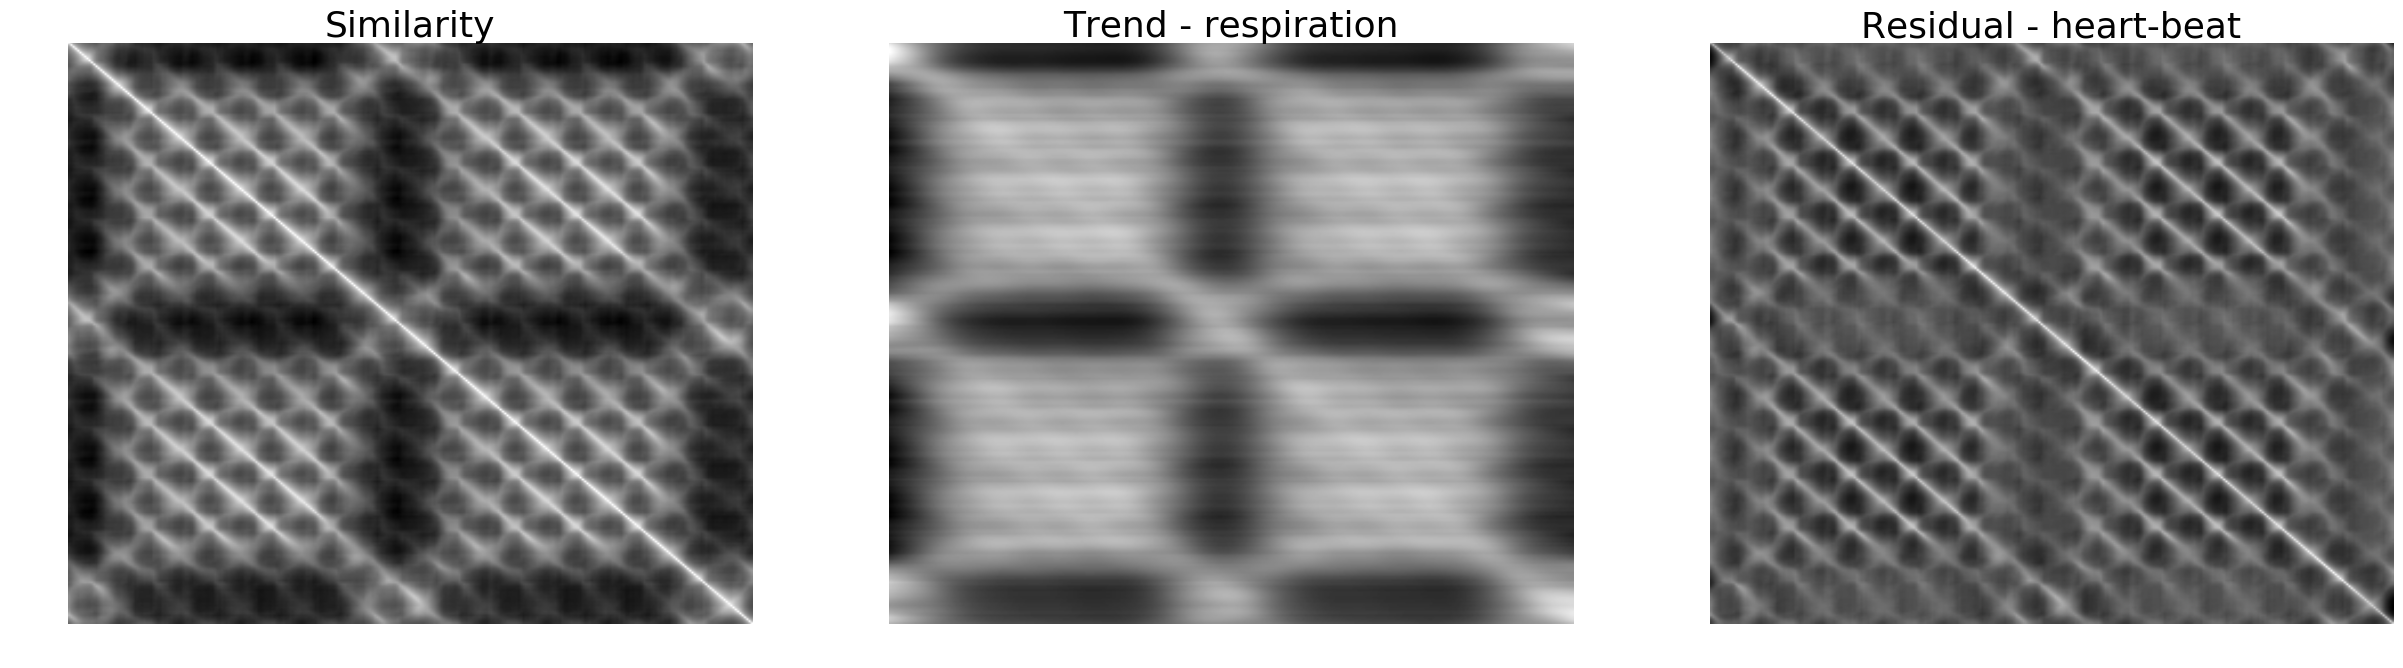
\includegraphics[width=4.0in]{figures/decoded/2015-07-27-10-36-06_2015-07-15-16-56-16_1.raw.bmode/simMat.png}
\ionbox{1.33in}\ionbox{1.33in}\ionbox{1.33in}\\
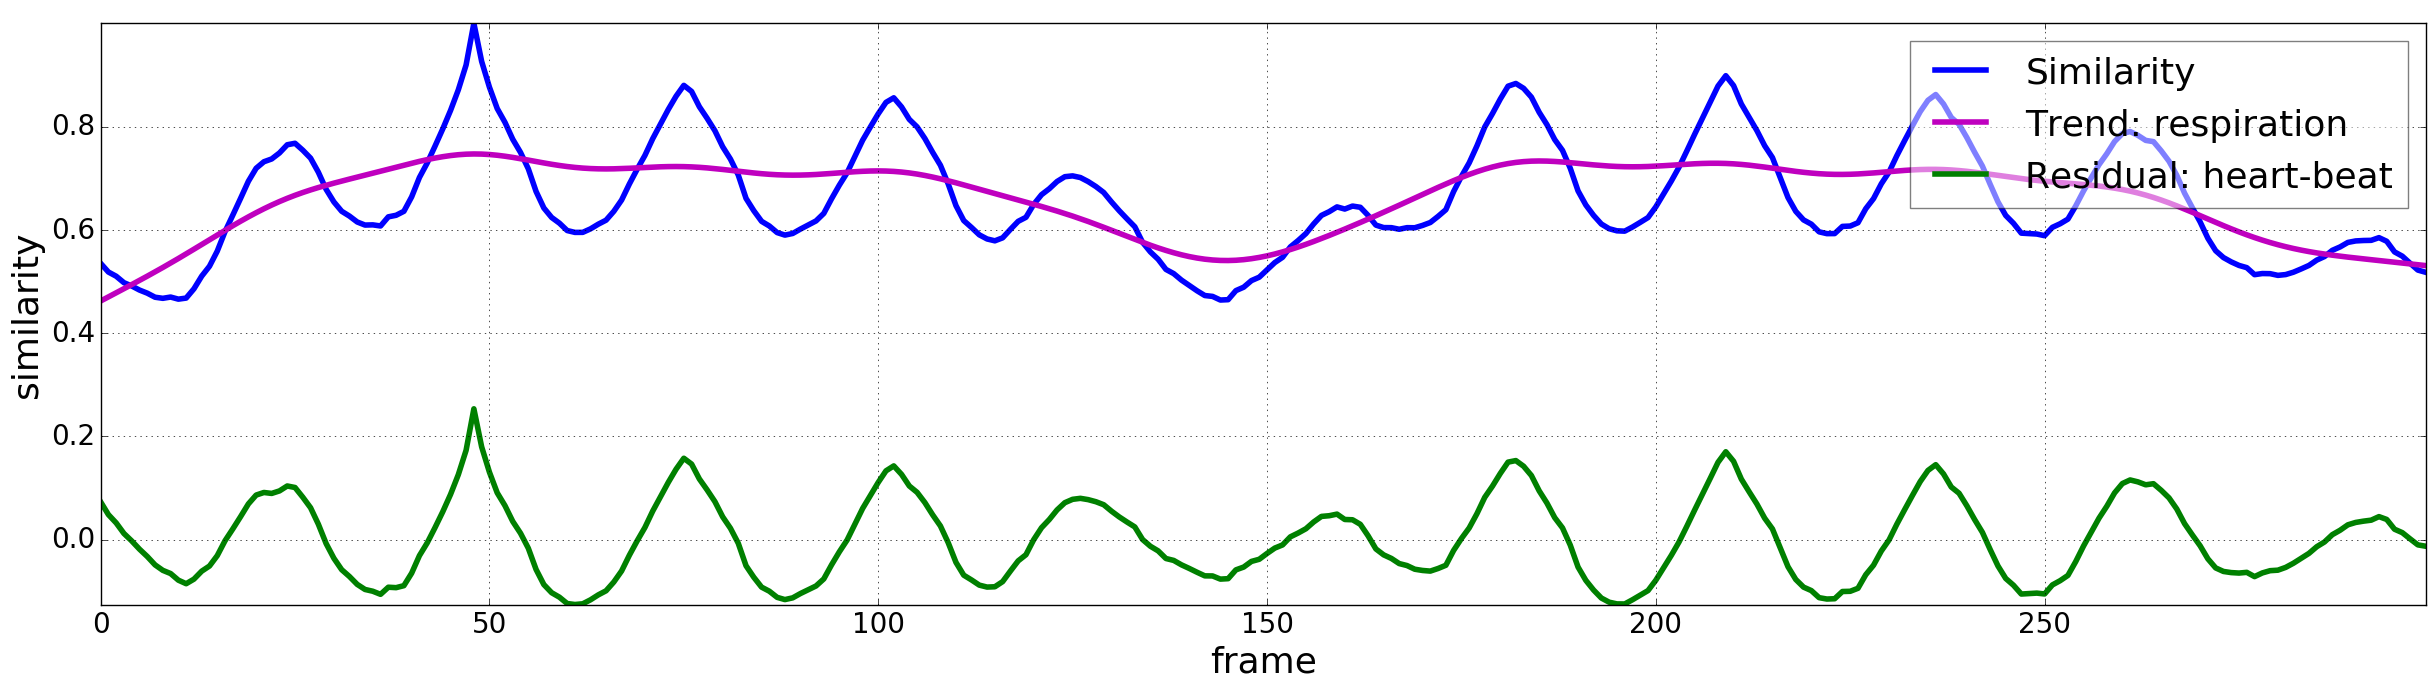
\includegraphics[width=4.25in]{figures/decoded/2015-07-27-10-36-06_2015-07-15-16-56-16_1.raw.bmode/season_trend_decomposition.png}
\ionbox{4.25in}\\
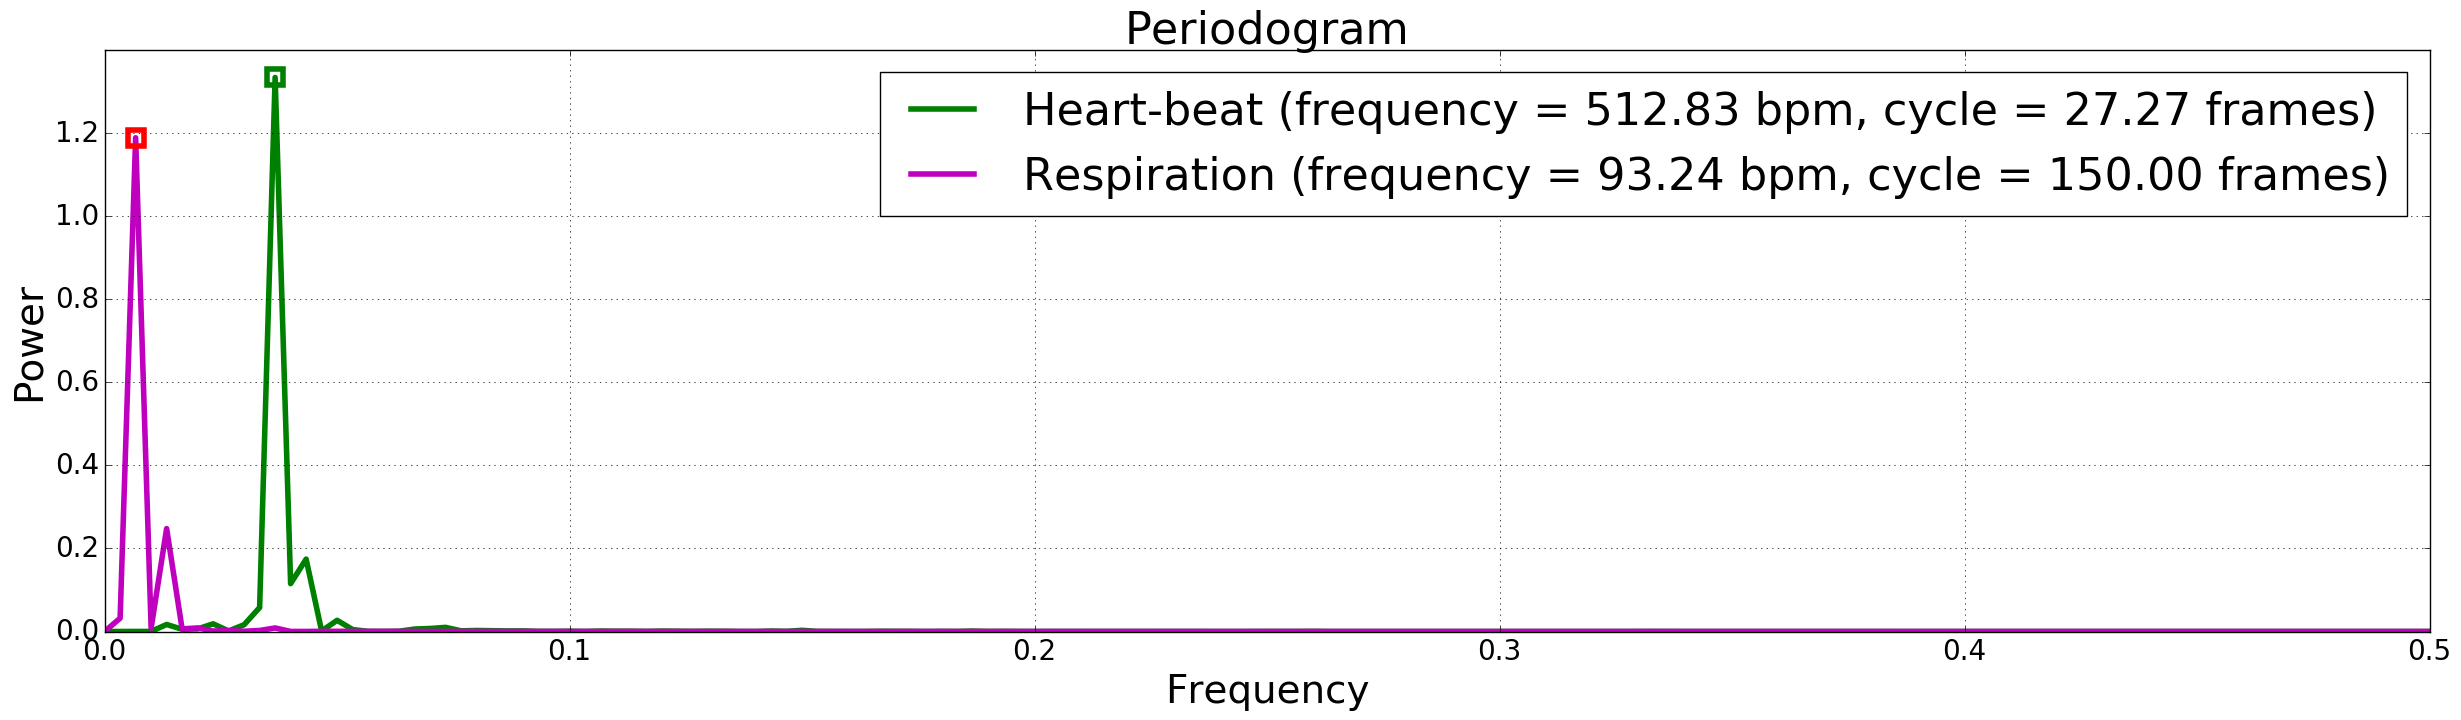
\includegraphics[width=4.25in]{figures/decoded/2015-07-27-10-36-06_2015-07-15-16-56-16_1.raw.bmode/periodogram.png}
\ionbox{4.25in}\\
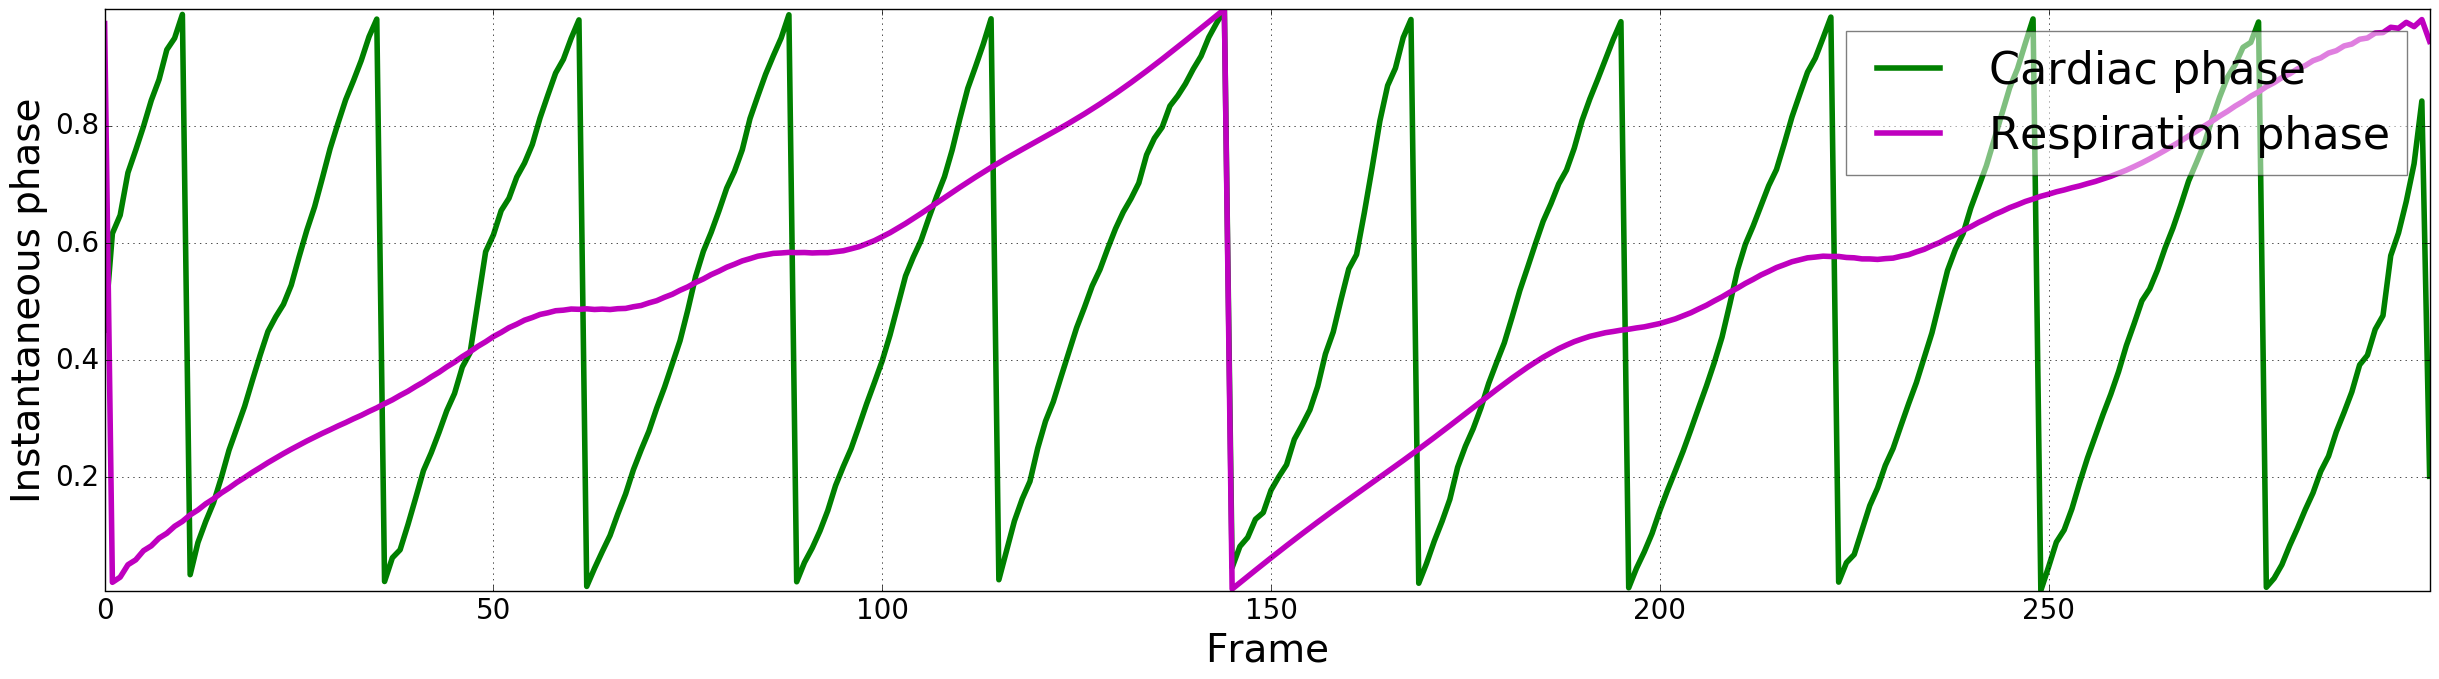
\includegraphics[width=4.25in]{figures/decoded/2015-07-27-10-36-06_2015-07-15-16-56-16_1.raw.bmode/instantaneous_phase.png}
\ionbox{4.25in}\\
%
\caption{Illustration of our phase estimation method: (a) Inter-frame similarity matrix, (b) Trend matrix corresponding to respiratory motion, (c) Residual matrix corresponding to beating heart motion, (d) Similarity profile chosen for phase estimation with associated trend/respiration and residual/heart-beat components, (e) Periodogram of heart-beat and respiration components along with periodicity characteristics (e.g. frequency, cycle duration) calculated from the dominant frequency, and (f) Instantaneous cardiac and respiratory phases estimated using the Hilbert transform.}
\label{fig:phase_estimation}
\end{IonFigT}
%
While there have been numerous efforts for the estimation of instantaneous phase and/or frequency in periodic univariate time series data\cite{Boashash1992,Lu2013,Luo2003}, there are not many methods that tackle this problem in a multivariate setting such as the case of periodic cardiac ultrasound videos wherein several thousands of variables (pixel intensities) are involved. Our strategy was to find a way to transforming this complex multi-variate problem into a univariate one and take advantage of existing univariate methods to solve the problem. 

	We first compute the similarity between all pairs of images/frames in the given periodic image sequence containing $N$ frames to create a symmetric matrix $A \in R^{N \times N}$ where in the element $A(i,j)$ is equal to the similarity between the $i^{th}$ and $j^{th}$ frames. Here in, we use normalized correlation also known as the Pearson correlation coefficient to quantify inter-frame similarity but, in principle, any of the similarity metrics used in image registration algorithms can potentially be chosen. Each row in the inter-frame similarity matrix $A$ can now be seen as a univariate time series. If the similarity metric is chosen with care and if the corresponding frame is not significantly corrupted, this time series can be expected to preserve the periodicity characteristics of the original image sequence. Two kinds of periodic motion are present in cardiac ultrasound videos, one corresponding to the beating heart motion and the other corresponding to respiratory motion. Figure \ref{fig:phase_estimation}(a) shows the inter-frame similarity matrix of one of our cardiac ultrasound videos wherein these two sources of periodicity can be clearly observed in many rows/columns. 

	Next, we use a trend extraction technique~\cite{Alexandrov2012} called the Hodrick-Prescott (HP) filter~\cite{Yamada2015}, widely used in econometrics, to decompose the frame similarity signal $u(t)$ corresponding to each row of $A$ into a sum of two components: (i) Trend component $\tau_{resp}(t)$ encompassing the periodicity characteristic of only the lower-frequency respiratory motion, and (ii) Residual component $r_{heart}(t)$ encompassing the periodicity characteristic of only the higher-frequency beating heart motion. The HP filter performs the decomposition of $u(t) = \tau_{resp}(t) + r_{heart}(t)$ by solving the following optimization problem:
\begin{equation}	
\argmin{\tau_{resp}(t)} \left[ \sum_{t=1}^{N}  \left(u(t) - \tau_{resp}(t) \right)^2  + \lambda \sum_{t=1}^{N-1} \left( \nabla^2 \tau_{resp}(t) \right)^2 \right] 
\end{equation}
where $\nabla^2\tau_{resp}(t) = \tau_{resp}(t+1) - 2 \tau_{resp}(t) + \tau_{resp}(t-1)$ is the second-order difference or derivative of the trend signal and $\lambda=6400$ is penalty parameter. Let $A_{resp}$ and $A_{heart}$ be the matrices whose rows contain the trend/respiratory and residual/heart-beat components, respectively, of the frame similarity signals in the corresponding rows of the similarity matrix $A$. Figures~\ref{fig:phase_estimation}(b,c) show the trend $A_{resp}$ and residual $A_{heart}$ matrices for one of our cardiac ultrasound videos. To minimize the effect of any noise on phase estimation, we pick frame similarity signal corresponding to the row of $A_{heart}$ whose periodogram or power-frequency distribution has minimum entropy. Let $\hat{u}(t)$ be the chosen frame similarity signal and let $\hat{\tau}_{resp}(t)$ and $\hat{r}_{heart}(t)$  be its associated trend/respiration and residual/heart-beat component signals, respectively. Figure~\ref{fig:phase_estimation}(d) shows the selected frame similarity signal (blue) along with the associated trend/respiration (pink) and residual/heart-beat (green) components. Figure~\ref{fig:phase_estimation}(e) shows the periodogram of these two components that are nicely segregated in frequency domain. The periodicity characteristics (e.g. frequency in beats-per-minute (bpm), cycle duration in frames, number of cycles) of heart-beat and respiration can be calculated based on the maximum-power frequency of their periodograms.
		
	Next, considering the narrow-band nature of the respiration and heart-beat signals (see  Figure~\ref{fig:phase_estimation}(e)), we use the Hilbert transform~\cite{Lu2013} to estimate the instantaneous phase of each frame. Specifically, we compute the instantaneous intra-period phase $\phi(t) \in \left [  -\pi, \pi\right )$ of a periodic time series $x(t)$ using its Hilbert transform $H_x(t)$ as follows: $\phi(t) = arctan \left( \frac{H_x(t)}{x(t)}\right)$ and map $\phi(t)$ from the range $\left [  -\pi, \pi\right )$ to $\left [  0, 1\right )$. Let $\hat{\phi}_{heart}(t)$ and $\hat{\phi}_{resp}(t)$ denote the instantaneous cardiac and respiratory phases computed from the trend/respiration $\hat{\tau}_{resp}(t)$ and residual/heart-beat $\hat{r}_{heart}(t)$ signals, respectively. Figure~\ref{fig:phase_estimation}(f) shows the instantaneous cardiac and respiratory phases computed from the heart-beat and respiration signals in Figure~\ref{fig:phase_estimation}(d). 
%
\vspace{-0.5cm}
\subsection{Gating out respiratory frames}
\label{sec:method:gating}
%
%
\begin{IonFigT}
\centering
%
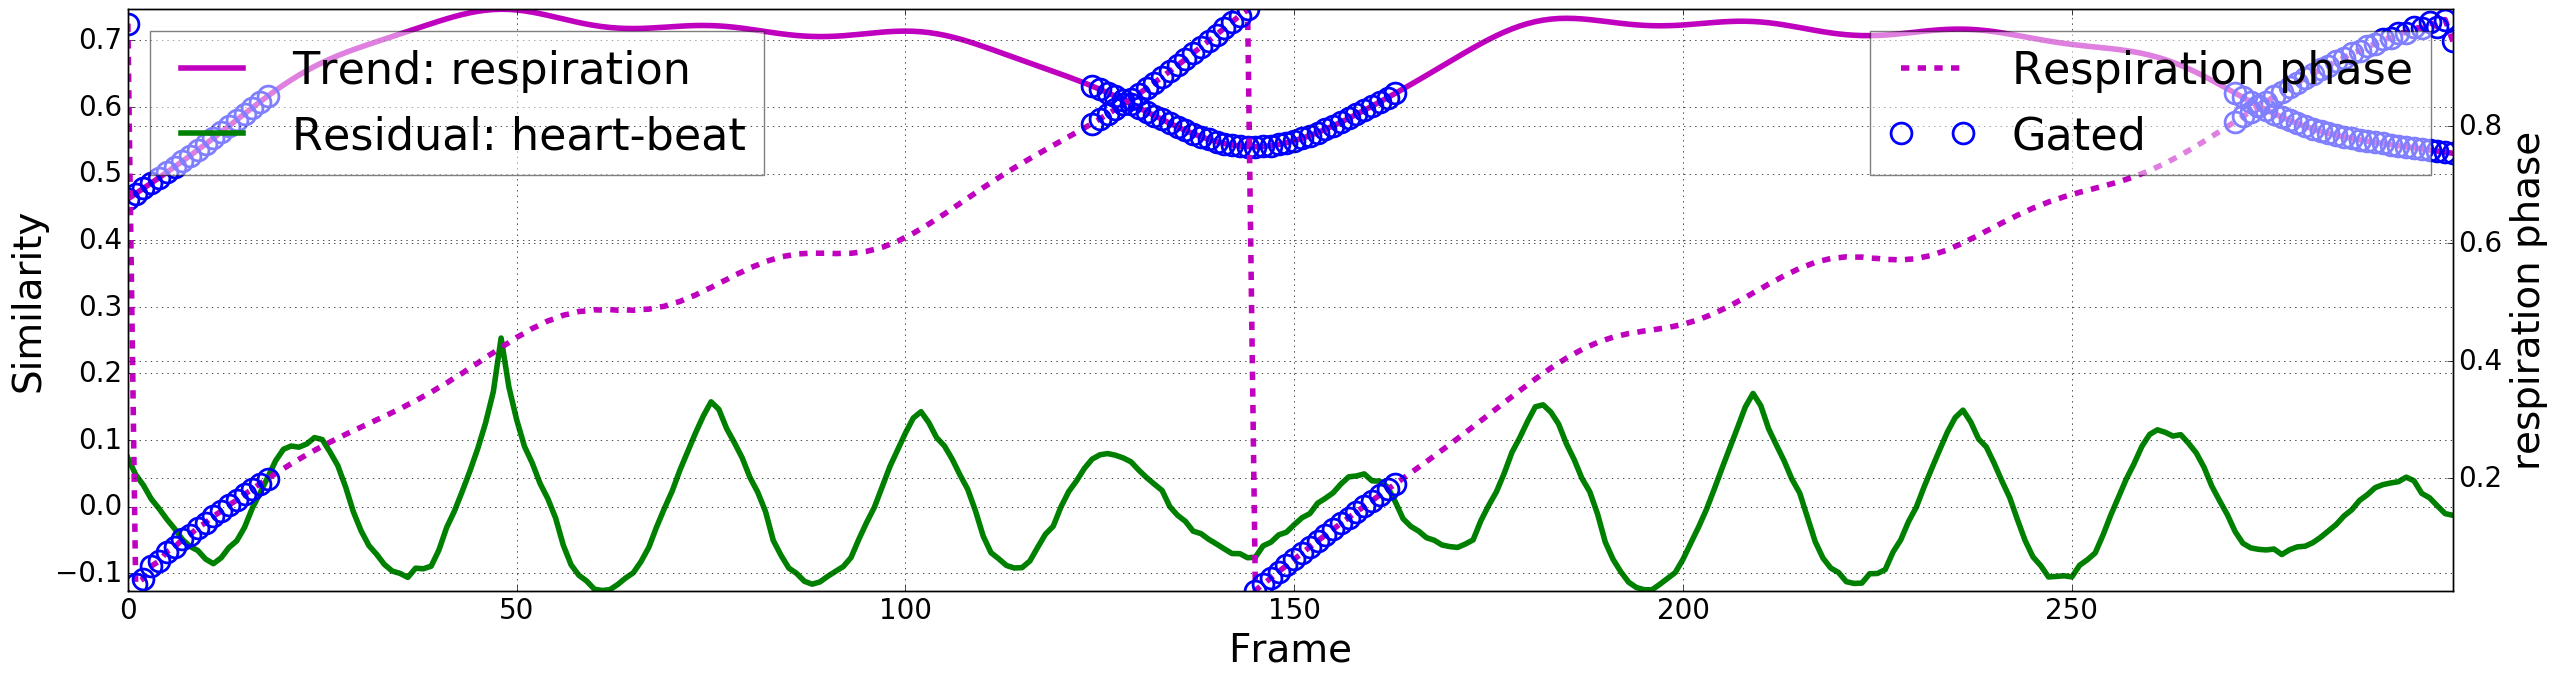
\includegraphics[width=4.25in]{figures/decoded/2015-07-27-10-36-06_2015-07-15-16-56-16_1.raw.bmode/respiratory_phase_gating.png}
\ionbox{4.25in}\\
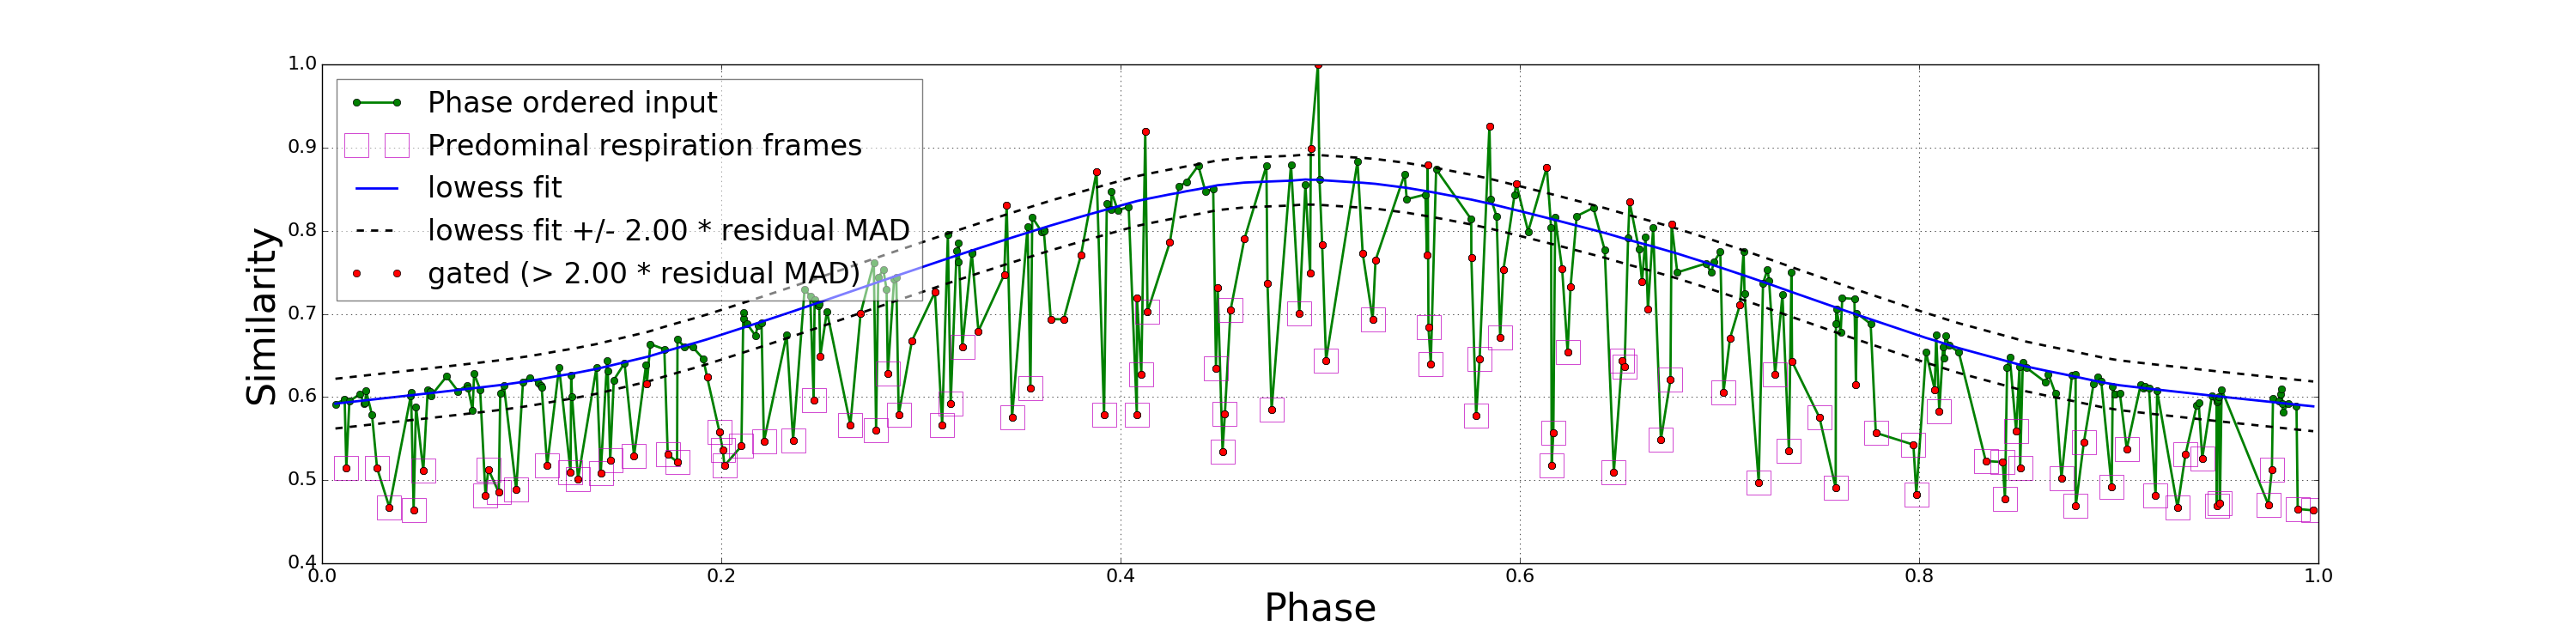
\includegraphics[width=4.25in]{figures/decoded/2015-07-27-10-36-06_2015-07-15-16-56-16_1.raw.bmode/robust_lowess_gating.png}
\ionbox{4.25in}\\
%
\caption{Illustration of our method for gating out respiratory frames: (a) Frames $F_{cutoff}$ discarded (blue circles) in the first step overlaid with the trend/respiration, residual/heart-beat, and instantaneous respiratory phase signals (b) residual/heart-beat signal $\hat{r}_{heart}(t)$ vs cardiac phase $\hat{\phi}_{heart}(t)$ overlaid with frames $F_{cutoff}$ discarded in step-1 (blue circle), LOWESS fit $L(\phi)$ (black solid), upper and lower bounds or 95\% confidence interval $(L(\phi) \pm 2.0 * \hat{\sigma}_L)$ of valid non-respiratory frames (black dotted), and frames $F_{resp}$ (red circles) gated at the end of step-2.}
\label{fig:respiratory_gating}
\end{IonFigT}
%
Once the cardiac and respiratory phases of each frame have been estimated, they can be used to filter out or guide the extraction of quantitative measurements from a desired part/point of the periodic cycle, a process commonly referred to as gating. In this section, we present a robust two-step method that uses these phase estimates to gate out video frames with significant respiratory motion.

	In the first step, based on the observation that respiratory motion mainly occurs around the minima of the trend/respiration signal $\hat{\tau}_{resp}(t)$ (pink curve in Fig.~\ref{fig:phase_estimation}(d)) with respiratory phase $\hat{\phi}_{resp}(t) = 0$, we perform a rough initial gating by discarding the frames $F_{cutoff} = \left \{ t \mid \hat{\phi}_{resp}(t) < c \parallel \hat{\phi}_{resp}(t) > (1 - c) \right \}$ whose phase distance from $\hat{\phi}_{resp}(t) = 0$ is below a specified cutoff value $c=0.2$. Figure~\ref{fig:respiratory_gating}(a) shows the discarded frames $F_{cutoff}$ overlaid on the trend/respiration $\hat{\tau}_{resp}(t)$, residual/heart-beat  $\hat{r}_{heart}(t)$, and respiratory phase $\hat{\phi}_{resp}(t)$ signals.
	
	In the second step, we learn a robust mapping $L(\phi) : \left [  0, 1\right ) \to R$ from cardiac phase to the residual/heart-beat component of the frame similarity signal by fitting a robust non-parametric regression model called Locally weighted regression (LOWESS) to the dataset $\left \{ \left(\hat{\phi}_{heart}(t), \hat{r}_{heart}(t) \right) \mid t \notin F_{cutoff}  \right \}$ containing the pair of the cardiac phase $\hat{\phi}_{heart}(t)$ and residual/heart-beat $\hat{r}_{heart}(t)$ signal values of all frames that do not belong to the set of frames $F_{cutoff}$ discarded in the first step above. Next, we compute a robust estimate of the standard deviation/dispersion $\hat{\sigma}_{L}$ of non-respiratory frames around the LOWESS fit based on the median absolute value of the difference between the LOWESS fit $L( \hat{\phi}_{heart}(t) )$ and residual/heart-beat signal $\hat{r}_{heart}(t)$ for all frames. Lastly, we gate out all frames $F_{resp} = \left \{ t \; \big\lvert \; \lvert L( \hat{\phi}_{heart}(t) ) - \hat{r}_{heart}(t)  \rvert   > k \times \hat{\sigma}_{L}  \right \}$ for which the absolute  difference between the LOWESS fit and heart-beat signal value is greater than $k = 2.0$ (95\% confidence interval) times the standard deviation $\hat{\sigma}_{L}$.	
%
\begin{IonFigT}
\centering
%
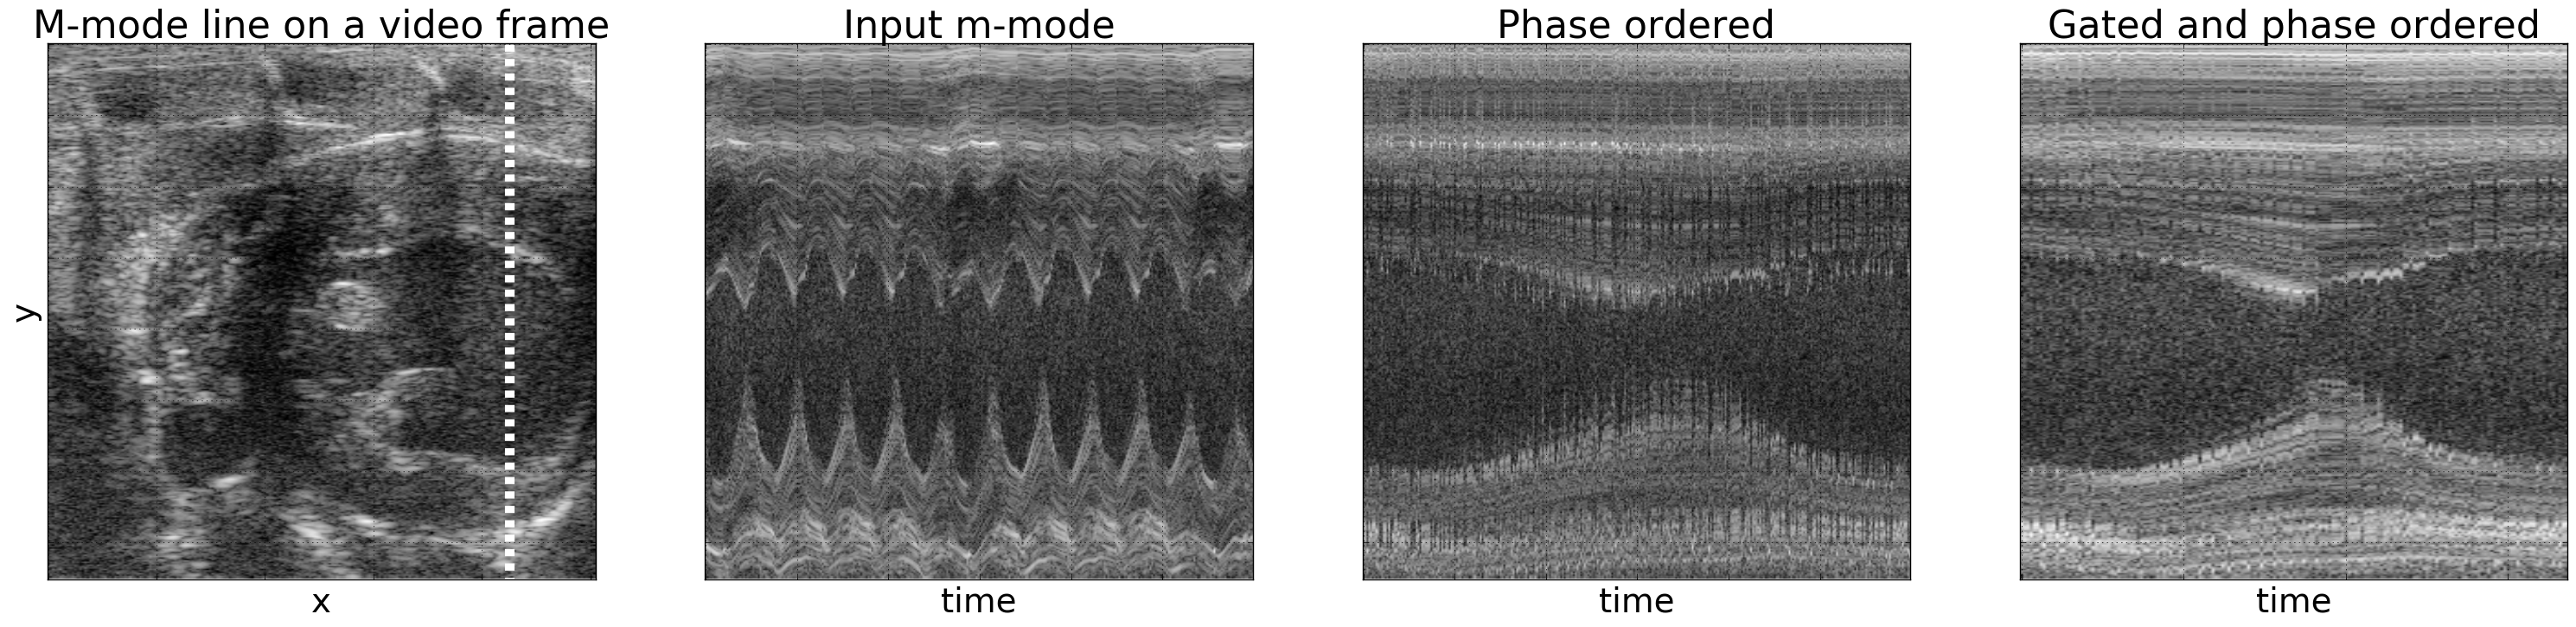
\includegraphics[width=4.5in]{figures/decoded/2015-07-27-10-36-06_2015-07-15-16-56-16_1.raw.bmode/phaseordered.png}
\ionbox{1.2in}\ionbox{1.1in}\ionbox{1.1in}\ionbox{1.1in}\\
%
\caption{Visualization of m-mode frames ordered by cardiac phase: (a) One of the frames in the video overlaid with the M-mode line shown in the next three images, (b) M-mode frames in the order they appear in the input video, (c) M-mode frames ordered by cardiac phase, and (d) Non-respiratory m-mode frames ordered by cardiac phase.}
\label{fig:phase_ordering}
\end{IonFigT}
%
\vspace{-0.5cm}
\subsection{Model to generate images by cardiac phase for super-resolution}
\label{sec:method:super_resolution}
%
In this section, we present a kernel regression model to reconstruct the image at any cardiac phase. This model can then be used to generate a single-cycle video representative of the subject's heart-beat at a higher temporal resolution.

Given a cardiac ultrasound video $I(t) : \{1, ..., N\} \to R^m$ of $N$ images with $m$ pixels each, we extract the residual/heart-beat component $\hat{r}_{heart}(t)$ of the frame similarity signal, estimate the instantaneous cardiac phase $\hat{\phi}_{heart}(t)$ of each frame, and compute the robust LOWESS fit $L(\phi) : \left [  0, 1\right ) \to R$ that maps cardiac phase to the heart-beat signal as  described in Sections~\ref{sec:method:phase_estimation} and ~\ref{sec:method:gating}. We then use Nadarya-Watson kernel regression\cite{Bishop2006} to learn a phase-parametrized image manifold in the form of a function $M(\phi): [0, 1) \to R^m $ that maps any cardiac phase $\phi$ to an image using kernel-weighted local average as follows:
\begin{equation}
M(\phi) = \frac{\sum_{t = 1}^{N} K \left( \phi, \hat{\phi}_{heart}(t) \right) I(t)}{\sum_{t = 1}^{n} K \left( \phi, \hat{\phi}_{heart}(t) \right)} 
\end{equation}
where kernel $K\left( \phi, \hat{\phi}_{heart}(t) \right) = exp\left \{ -\frac{ \mid \phi - \hat{\phi}_{heart}(t) \mid^2}{2  \sigma^2_\phi} \right \} \times exp\left \{ -\frac{ \mid L(\phi) - \hat{r}_{heart}(t) \mid^2}{2  \sigma^2_{L}} \right \}$ is defined as the product of two radial-basis function (RBF) kernels. The first RBF kernel  weighs images inversely proportional to their distance (accounting for periodicity) in the cardiac phase space. Its bandwidth $\sigma_\phi$ is set equal to a constant $k_\phi = 0.4$ times the median difference in cardiac phase between consecutive frames of the given image sequence. The second RBF kernel weighs images inversely proportional to their deviation from the LOWESS prediction $L(\phi)$ in the residual/heart-beat signal space. Its bandwidth $\sigma_{L}$ is set equal to a constant $k_L = 2.0$ times the robust estimate of standard deviation/dispersion $\hat{\sigma}_{L}$ of non-respiratory frames around the LOWESS fit as described in Section~\ref{sec:method:gating}. A single-cycle video representative of the subject's heart-beat can now be reconstructed by sampling the manifold $M(\phi)$ at any desired resolution. 
\vspace{-0.5cm}
\section{Results}
\label{sec:results}
%
We use cardiac ultrasound videos and associated ECG recordings of 6 mice to validate our methods. The ultrasound videos were acquired using the VisualSonics Vevo 2100 scanner at 233 frames per second. Each video consists of approximately 300 frames, 11 cardiac cycles, and 2 respiratory cycles.

	We validate the cardiac phase estimates of our method by comparing them with the ECG signal which is the gold standard for cardiac gating. Figure~\ref{fig:instaphase_vs_ecg}(a) shows a head-to-head comparison between the ECG signal and the cardiac phase signal obtained using the method described in Section~\ref{sec:method:phase_estimation} for one of the 6 videos. Notice how well the locations of the  QRS peaks (red circles) in the ECG signal and the corresponding minima (black circles) of the cardiac phase signal in each cycle match. Table 1 reports the $R^2$ correlation and the $mean \pm std$ error between the locations of the QRS peaks and the corresponding minima of the cardiac phase signals for all 6 videos. Figure~\ref{fig:instaphase_vs_ecg}(b) presents a visual comparison of five video frames evenly spaced in time between two consecutive QRS peaks (top-row) and corresponding minima of the cardiac phase signal (bottom-row). Notice the high-level of similarity in the images of each column.  Figure~\ref{fig:phase_ordering}(b,c) shows the frames of an m-mode line before and after ordering with the estimated cardiac phase. Figure~\ref{fig:phase_ordering}(d) shows m-mode frames ordered by cardiac phase after gating out respiratory frames. The supplementary material includes a video showing the estimated cardiac and respiratory phases of each frame for one of our datasets.
	
	We validate the accuracy of our kernel regression model for reconstructing images at any cardiac phase using leave-one-out-cross-validation (LOOCV). In each round of cross-validation, we randomly exclude one of the non-respiratory frames in the video, fit our kernel-regression model on the remaining frames, use the fitted model to reconstruct the image at the cardiac phase of the excluded frame, and compute the similarity between the reconstructed and original image using normalized correlation. The second column of Table~\ref{table:image_reconstruction} shows the $mean \pm std$ of normalized correlation between the reconstructed and the original images over 50 rounds of LOCCV for all 6 videos. As a baseline, the third column of  Table~\ref{table:image_reconstruction} shows the $mean \pm std$ of the normalized correlation between frames at QRS peaks of the ECG signal. The supplementary material includes single-cycle videos at 2x and 4x temporal resolution generated using the kernel regression model wherein the motion of heart chambers and valves is much clear than the original video. 
%
%
\begin{table}[t]
\begin{minipage}[t]{0.45\linewidth}
\centering
\caption{Comparision between frame positions of the QRS peaks in ECG signal and the corresponding minima of the estimated cardiac phase for 6 videos.}
\begin{tabular}{|c|c|c|}
\hline
\multicolumn{1}{|l|}{} & \multicolumn{2}{l|}{QRS peak frame identification} \\ \hline
VID & $R^2$ & $mean \pm std \; error$ \\ \hline
1 & \; 0.9995 \; & 1.55 $\pm$ 0.89 \\ \hline
2 & \; 0.9995 \; & 1.36 $\pm$ 1.15 \\ \hline
3 & \; 0.9996 \; & 1.45 $\pm$ 0.89 \\ \hline
4 & \; 0.9998 \; & 0.73 $\pm$ 0.62 \\ \hline
5 & \; 0.9990 \; & 2.09 $\pm$ 1.78 \\ \hline
6 & \; 0.9992 \; & 1.40 $\pm$ 1.74 \\ \hline
\end{tabular}
\label{table:phase_estimation}
\end{minipage}
%
\hspace{0.5cm}
%
\begin{minipage}[t]{0.45\linewidth}
\caption{Evaluation of our kernel regression model for reconstructing images at any cardiac phase using 50 rounds of Leave one out cross-validation (LOOCV) for 6 videos.}
\centering
\begin{tabular}{|c|c|c|}
\hline
\begin{tabular}[c]{@{}c@{}}VID \\ $\;$ \end{tabular} & \begin{tabular}[c]{@{}c@{}}LOOCV (50)\\ $mean \pm std \; ncorr$\end{tabular} & \begin{tabular}[c]{@{}c@{}}QRS Peak Frames\\ $mean \pm std \; ncorr$\end{tabular} \\ \hline
1 & 0.8562 $\pm$ 0.0366 & 0.7981 $\pm$ 0.0532 \\ \hline
2 & 0.8558 $\pm$ 0.0525 & 0.7877 $\pm$ 0.0503 \\ \hline
3 & 0.8592 $\pm$ 0.0348 & 0.7849 $\pm$ 0.0457 \\ \hline
4 & 0.8713 $\pm$ 0.0348 & 0.8395 $\pm$ 0.0486 \\ \hline
5 & 0.8655 $\pm$ 0.0312 & 0.8196 $\pm$ 0.0476 \\ \hline
6 & 0.8736 $\pm$ 0.0278 & 0.8270 $\pm$ 0.0778 \\ \hline
\end{tabular}
\label{table:image_reconstruction}
\end{minipage}
\vspace{-0.3cm}
\end{table}
%
%
\vspace{-0.5cm}
\section{Conclusion}
\label{sec:conclusion}
%
In this paper, we have presented a novel method to estimate the instantaneous cardiac and respiratory phases directly from the cardiac ultrasound video. We have also presented a robust non-parametric regression technique for gating out respiratory frames and a novel kernel regression model for reconstructing images at any cardiac phase to facilitate temporal super-resolution. Having demonstrated a proof of concept, we next plan to evaluate our methods on more datasets, especially of subjects with irregular heart beats, and address any remaining pitfalls. One drawback of our phase estimation method is a strong assumption of periodicity which may breakdown in the case of subjects with cardiac arrhythmia. To address this, we will look into generalizations of the hilbert transform\cite{Lu2013} that are more susceptible noise. Another drawback is that the use normalized correlation to measure inter-frame similarity relies on an inherent assumption that a large part of the image is pulsating. To relax this, we will try to devise more sophisticated local patch-based similarity measures. We encourage the readers to watch the supplementary videos for a better understanding of the effectiveness and utility of the proposed methods. 
%
\vspace{-0.5cm}
\bibliographystyle{splncs03}
\bibliography{library}
\end{document}







